%
%
%
%
Esse capítulo tem uma proposta mais direta, aqui trataremos de alguns poucos comandos diretos para Manipulação de Dados, ou \textbf{DML}.

Para prosseguir, vamos primeiro popular nosso banco de dados com valores iniciais. Buscando simplicidade, nesta sessão focaremos nossos exemplos ao redor da tabela \texttt{Especialidades}. Todavia, é possível visualizar os dados inseridos nas demais na sessão de Apêndice (\textbf{Cap. \ref{subsec: DML} p. \pageref{subsec: DML}}). 

Usando o comando \texttt{INSERT} inserimos dados no campo \texttt{nome} e \texttt{descricao}:

\begin{lstlisting}[
    language=MySQL,
    caption=Perceba que não precisamos colocar valor para \texttt{id\_especialidade} por causa da opção \texttt{AUTO\_INCREMENT},
    label=insert_especialidade
]
INSERT INTO Especialidades 
    (nome, descricao) 
VALUES
    ('Cardiologia', 'Especialidade medica que trata doencas do coracao e sistema circulatorio'),
    ('Dermatologia', 'Especialidade medica que trata doencas da pele, cabelos e unhas'),
    ('Pediatria', 'Especialidade medica dedicada ao cuidado de criancas e adolescentes'),
    ('Ortopedia', 'Especialidade medica que trata doencas e deformidades do sistema musculoesqueletico'),
    ('Ginecologia', 'Especialidade medica que trata da saude do sistema reprodutor feminino'),
    ('Clinico Geral', 'Medico generalista que trata de problemas de saude diversos'),
    ('Campo para teste', 'Usaremos esse campo para testar os demais comandos');
\end{lstlisting}

Vamos agora mudar o nome do dado "Campo para Teste" para apenas "Teste". Antes disso, vamos verificar se ele foi inserido com sucesso, para isso, basta usarmos \texttt{SELECT * FROM Especialidades WHERE nome='Campo para teste';} :

\begin{figure}[H]
    \centering
    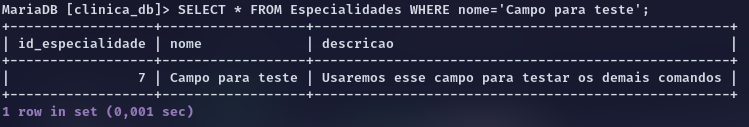
\includegraphics[width=1\linewidth]{Text//DML/campo_teste.png}
    \caption{\texttt{Campo para teste} antes das alterações}
    \label{fig:CampoTeste1}
\end{figure}

Agora, usando \texttt{UPDATE} alteraremos o nome:

\begin{lstlisting}[
    language=MySQL,
    caption=UPDATE nome,
    label=Update_especialidade
]
UPDATE Especialidades 
    SET nome = 'Teste'
WHERE
    nome = 'Campo para teste';;
\end{lstlisting}

Assim:

\begin{figure}[H]
    \centering
    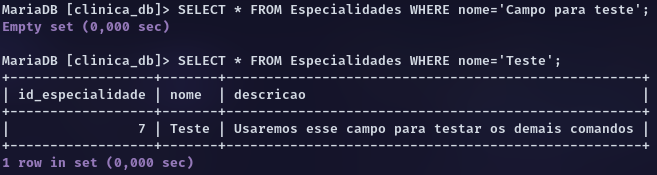
\includegraphics[width=1\linewidth]{Text//DML/campo_teste2.png}
    \caption{Perceba que não existe mais um dado com nome "Campo para Teste" pois o mesmo mudou para "Teste"}
    \label{fig:CampoTeste2}
\end{figure}

Finalmente vamos apagar o campo que mudamos, para isso basta usarmos \texttt{DELETE}:
\begin{lstlisting}[
    language=MySQL,
    caption=DELETE Teste,
    label=Update_especialidade
]
DELETE FROM Especialidades WHERE nome = 'Teste';
\end{lstlisting}

E então não temos mais esse registro em nossa tabela:

\begin{figure}[H]
    \centering
    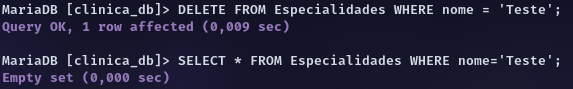
\includegraphics[width=1\linewidth]{Text/DML/Delete_teste.png}
    \caption{A ausência do valor no output indica que o dado não existe.}
\end{figure}
